\documentclass[12pt]{article}
\usepackage[english]{babel}
\usepackage[utf8x]{inputenc}
\usepackage{amsmath}
\usepackage{hyperref} 
\usepackage{subfigure}
\usepackage{graphicx, float}
\usepackage[colorinlistoftodos]{todonotes}

\begin{document}
	
	\begin{titlepage}
		
		\newcommand{\HRule}{\rule{\linewidth}{0.5mm}} % Defines a new command for the horizontal lines, change thickness here
		
		\center % Center everything on the page
		
		%----------------------------------------------------------------------------------------
		%	HEADING SECTIONS
		%----------------------------------------------------------------------------------------
		
		\textsc{\LARGE Central Washington University}\\[1.5cm] % Name of your university/college
		\textsc{\Large Computational Intelligence}\\[0.5cm] % Major heading such as course name
		\textsc{\large Winter 2019}\\[0.5cm] % Minor heading such as course title
		
		%----------------------------------------------------------------------------------------
		%	TITLE SECTION
		%----------------------------------------------------------------------------------------
		
		\HRule \\[0.4cm]
		{ \huge \bfseries Project 3 Report}\\[0.4cm] % Title of your document
		\HRule \\[1.5cm]
		
		%----------------------------------------------------------------------------------------
		%	AUTHOR SECTION
		%----------------------------------------------------------------------------------------
		
		\begin{minipage}{0.4\textwidth}
			\begin{flushleft} \large
				\emph{Author:}\\
				Hermann \textsc{Yepdjio} % Your name
			\end{flushleft}
		\end{minipage}
		~
		\begin{minipage}{0.4\textwidth}
			\begin{flushright} \large
				\emph{Professor:} \\
				Dr. Razvan \textsc{Andonie} % Supervisor's Name
			\end{flushright}
		\end{minipage}\\[1cm]
		
		% If you don't want a supervisor, uncomment the two lines below and remove the section above
		%\Large \emph{Author:}\\
		%John \textsc{Smith}\\[3cm] % Your name
		
		%----------------------------------------------------------------------------------------
		%	DATE SECTION
		%----------------------------------------------------------------------------------------
		
		{\large \today}\\ % Date, change the \today to a set date if you want to be precise
		
		%----------------------------------------------------------------------------------------
		%	LOGO SECTION
		%----------------------------------------------------------------------------------------
		
		
\includegraphics[width=12cm]{CWU-Logo.png}\\[.5cm] % Include a department/university logo - this will require the graphicx package
		
		%----------------------------------------------------------------------------------------
		
		\vfill % Fill the rest of the page with whitespace
		
	\end{titlepage}
	\newpage
	\tableofcontents
	\newpage
	
	
	
	\section{Problem Description}
	The genetic algorithm is a technique used for solving optimization problems. It follows the same process that drives biological evolution. It starts with an initial population of solutions which it modifies at each step to produce a new generation of the population usually better than the previous generation. The modification of the population is done through processes such as cross-overs and mutations.
	
	The purpose of this project was to implement a genetic algorithm able to generate a magic square of size n. A magic square of size n is an n*n matrix which contains unique numbers from 1 to $n^2$ and with each column, row and diagonal having the same sum. After implementing the algorithm, we experimented using different sizes for the population and different mutation rates. The details of the implementation as well as the results of the experimentation are discussed below.
	
	\section{Implementation}
		\subsection{Input Data}
			The program takes the following inputs from the user before the search can start:
			\begin{itemize}
				\item an integer greater than 3 for the size of the magic square (3 for 3*3, 4 for 4*4 etc ...),
				\item an integer for the size of the initial population (the size of the population remains constant across generations),
				\item a float number between 0 and 1 for the mutation rate
			\end{itemize}
		
		\subsection{Selection}
			For the crossover operation, a mating pool of half the size of the population is created and filled with chromosomes from the original population selected based on some probabilities calculated using their fitness.
		\subsection{Crossover}
			Since a magic square requires all numbers of the matrix to be unique, simple crossover techniques such as taking halves of the genes of 2 parents and merge them together to produce an offspring could not be considered. Therefore, we used an approach proposed on the paper \href{http://www.ceng.metu.edu.tr/~ucoluk/research/publications/tspnew.pdf}{Genetic Algorithm Solution of the TSP Avoiding Special Crossover and Mutation} written by Göktürk Üçoluk. The approach basically follows the following steps to produce 2 offspring:
			
			\begin{itemize}
				\item calculate the inversion sequence for each parent,
				\item generate the children arrays,
				\item transforming the children arrays back to permutation representation.
			\end{itemize}
		The paper mentioned above provides more details on how those steps are performed.
		
		\subsection{Mutation}
		After the crossover is performed, the program randomly decides whether to apply a mutation or not based on the mutation rate provided by the user. After the mutation stage is over (no matter if genes were mutated or not) the program looks for the least two fitted chromosomes in the original population and replace them with the new children.
	\section{Experimentation}
		\subsection{Process}
			During this stage, we experimented generating magic squares of different sizes using different mutation rates and population sizes. The results were recorded and are described in the next subsection.
		\subsection{results}
			\begin{figure}[H]
				\hfill
				\subfigure[3*3 Magic Square Evolution of Fittest Chromosome]{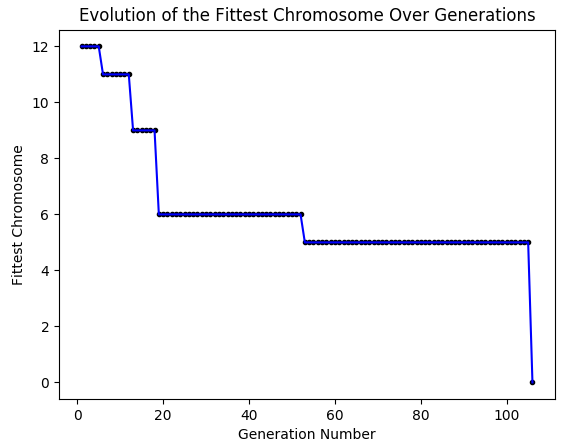
\includegraphics[width=6cm]{3_3_fittest.png}}
				\hfill
				\subfigure[3*3 Magic Square Evolution of the Average  Fitness]{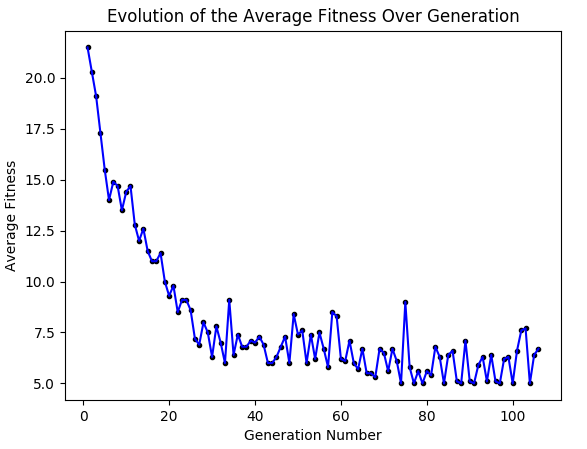
\includegraphics[width=6cm]{3_3_avg.png}}
				\hfill
				\caption{3*3 Magic Square. pop\_size = 10, mutation rate = 0.5}
			\end{figure}
		
			\begin{figure}[H]
				\hfill
				\subfigure[4*4 Magic Square Evolution of Fittest Chromosome]{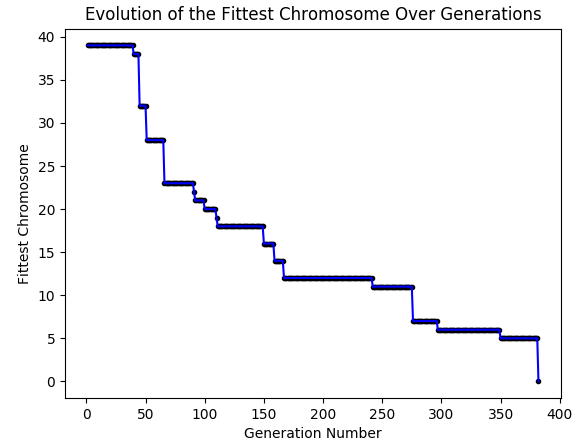
\includegraphics[width=6cm]{4_4_fittest.png}}
				\hfill
				\subfigure[4*4 Magic Square Evolution of the Average  Fitness]{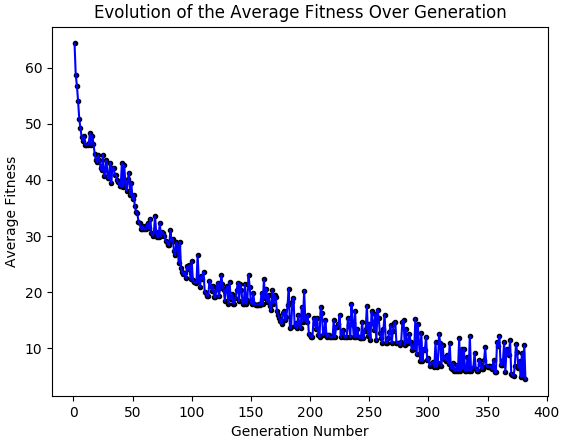
\includegraphics[width=6cm]{4_4_avg.png}}
				\hfill
				\caption{4*4 Magic Square. pop\_size = 10, mutation rate = 0.5}
			\end{figure}
		
			In Figures 1 and 2 above we can see that a 3*3 and a 4*4 magic squares were found (fitness = 0) at $generation\simeq100 $ for the first and $generation\simeq 400$ for the second. We can also see that both the fitness of the fittest chromosome and the average fitness of the population improve (get closer to 0) over the generations.
			\begin{figure}[H]
				\hfill
				\subfigure[5*5 Magic Square Evolution of Fittest Chromosome]{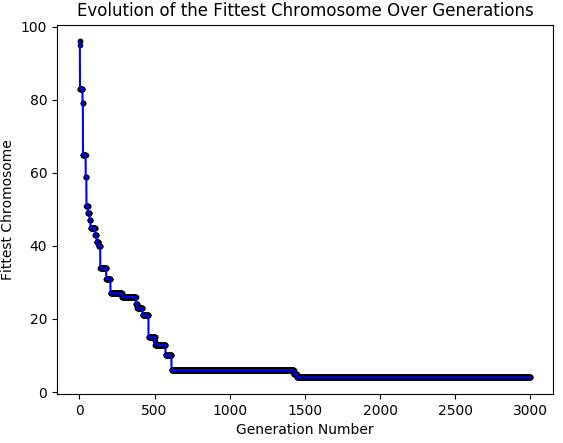
\includegraphics[width=6cm]{5_5_fittest.png}}
				\hfill
				\subfigure[5*5 Magic Square Evolution of the Average  Fitness]{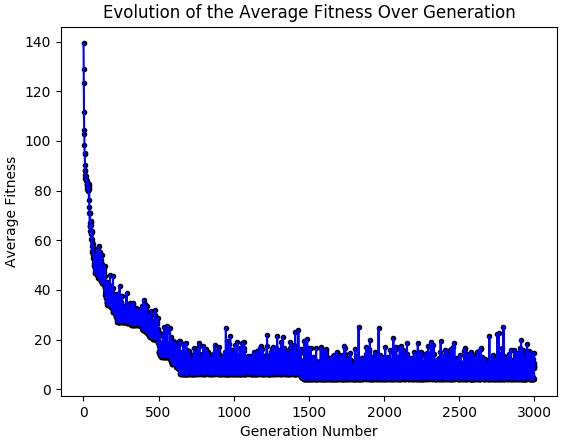
\includegraphics[width=6cm]{5_5_avg.png}}
				\hfill
				\caption{5*5 Magic Square. pop\_size = 10, mutation rate = 0.5}
			\end{figure}
			
			In Figure 3 we can see the same convergence of the average fitness and fitness of the fittest chromosome observed in Figures 1 and 2 even though a solution is not found before reaching generation 3000.
			\begin{figure}[H]
				\hfill
				\subfigure[5*5 Magic Square Evolution of Fittest Chromosome]{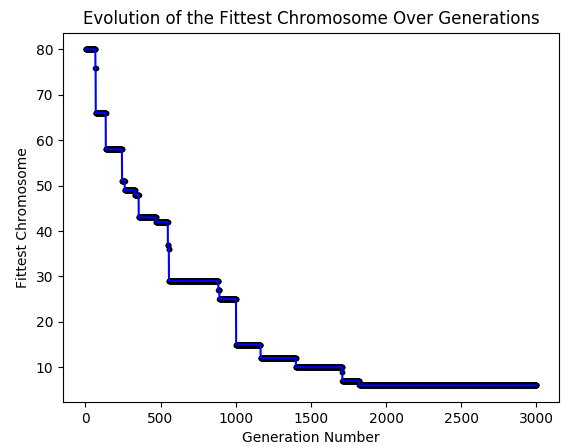
\includegraphics[width=6cm]{5_5_fittest_100.png}}
				\hfill
				\subfigure[5*5 Magic Square Evolution of the Average  Fitness]{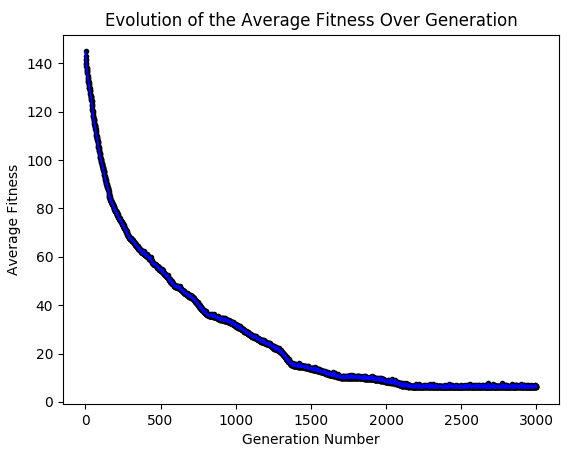
\includegraphics[width=6cm]{5_5_avg_100.png}}
				\hfill
				\caption{5*5 Magic Square. pop\_size = 100, mutation rate = 0.5}
			\end{figure}
		
			Figures 4 shows that the same convergence observed in Figure 3 happens when we increase the population size from 10 to 100. However, this convergence occurs more slowly than it does in Figure 3.
			\begin{figure}[H]
				\hfill
				\subfigure[5*5 Magic Square Evolution of Fittest Chromosome]{\includegraphics[width=6cm]{{5_5_fittest_0.1}.png}}
				\hfill
				\subfigure[5*5 Magic Square Evolution of the Average  Fitness]{\includegraphics[width=6cm]{{5_5_avg_0.1}.png}}
				\hfill
				\caption{5*5 Magic Square. pop\_size = 10, mutation rate = 0.1}
			\end{figure}
		
			Figure 5 shows that reducing the mutation rate from 0.5 to 0.1 affect the speed at which the solutions converge and therefore also affect the optimal solution that can be found given a limited number of generations.
			\begin{figure}[H]
				\hfill
				\subfigure[5*5 Magic Square Evolution of Fittest Chromosome]{\includegraphics[width=6cm]{{5_5_fittest_0.01}.png}}
				\hfill
				\subfigure[5*5 Magic Square Evolution of the Average  Fitness]{\includegraphics[width=6cm]{{5_5_avg_0.01}.png}}
				\hfill
				\caption{5*5 Magic Square. pop\_size = 10, mutation rate = 0.01}
			\end{figure}
			
			Figure 6 basically shows the same results observed in Figure 5.
			\begin{figure}[H]
				\hfill
				\subfigure[10*10 Magic Square Evolution of Fittest Chromosome]{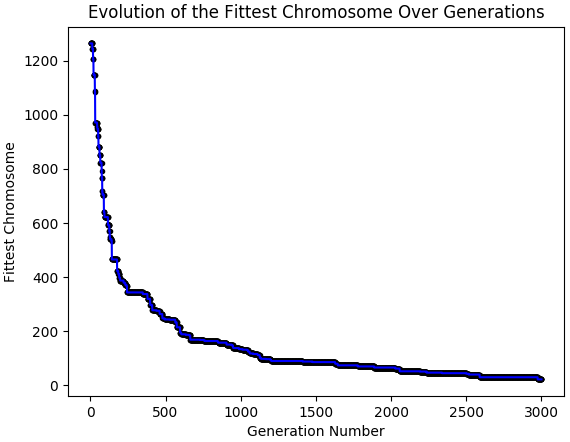
\includegraphics[width=6cm]{10_10_fittest.png}}
				\hfill
				\subfigure[10*10 Magic Square Evolution of the Average  Fitness]{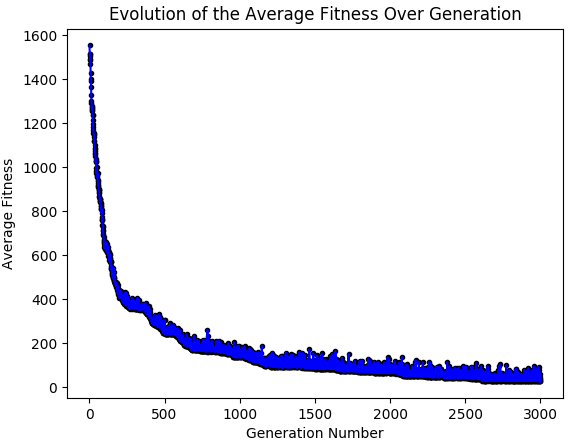
\includegraphics[width=6cm]{10_10_avg.png}}
				\hfill
				\caption{10*10 Magic Square. pop\_size = 10, mutation rate = 0.5}
			\end{figure}
		
			Figure 7 shows how the solutions converge for a 10*10 magic square. We can see a huge improvement for the average fitness from above 1500 at generation 0 to less than 50 at generation 3000.
	\section{Conclusion}
		From the experimentation described above, we can conclude that choosing values for parameters such as the mutation rate or the population size depends on the type of problem  we are trying to solve. Even though in general having a large population and a small mutation rate produces better results, in some cases like ours, that assumption does not hold true as we got better results using a small population size and a large mutation rate. However, figuring out what type of values we should use can only be done through experimenting with different values and observe which ones work better.  
	
	
\end{document}